
\chapter{Appendix}
\section{Dataset Introduction} 	

\begin{figure}[htbp]
	\centering
	\begin{subfigure}[b]{0.48\textwidth}
		\centering
		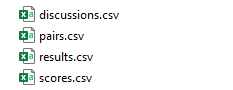
\includegraphics[width=\textwidth]{figure/dataset_structure}
		\caption{}
		\label{fig: datasetstructure}
	\end{subfigure}
	\hfill
	\begin{subfigure}[b]{0.48\textwidth}
		\centering
		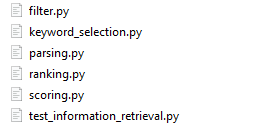
\includegraphics[width=\textwidth]{figure/code_structure}
		\caption{}
		\label{fig: codestructure}
	\end{subfigure}
	\hfill
	\caption[]{(a) Prepared dataset structure. (b) Code module structure.}
	\label{fig: structures}
\end{figure}

There are four parts of the dataset as shown in figure \ref{fig: datasetstructure} : 
\begin{itemize}
	\item \textbf{discussions} contains document ids, discussion ids, and text of discussions,
	\item \textbf{results} contains document ids, result ids, and text of results, 
	\item \textbf{pairs}  contains document ids, discussion ids, and result ids, 
	\item \textbf{scores}  contains document ids of result paragraphs, result ids, document ids of discussion paragraphs, discussion ids, scores.			
\end{itemize}				

An example of the dataset created for scoring the result paragraphs and discussion paragraphs ("scores" part of the dataset) is shown in table \ref{tab: result_discussion_score}.

\begin{table}[htbp]
	\centering
	\begin{tabular}{rrrrr}
		\toprule
		\multicolumn{1}{l}{doc\_id\_result} & \multicolumn{1}{l}{result\_id} & \multicolumn{1}{l}{doc\_id\_discussion} & \multicolumn{1}{l}{discussion\_id} & \multicolumn{1}{l}{score} \\
		\midrule
		1421389 & 0     & 1421389 & 0     & 4 \\
		1421389 & 0     & 1421389 & 3     & 2 \\
		653044 & 1     & 653044 & 2     & 4 \\
		2442696 & 1     & 2442696 & 1     & 2 \\
		2442696 & 1     & 193334 & 5     & 0 \\
		363993 & 1     & 363993 & 1     & 4 \\
		363993 & 1     & 363993 & 2     & 2 \\
		360628 & 1     & 363993 & 1     & 1 \\
		363993 & 1     & 995302 & 2     & 2 \\
		\midrule
		&       &       &       &  \\
	\end{tabular}%
	\caption{An example of the result and discussion scores.}
	\label{tab: result_discussion_score}%
\end{table}%

For each paper, an id to every result paragraph and discussion paragraph is given, and these result and discussion paragraphs are manually scored, i.e. pair result paragraphs to discussion paragraphs. 
For example, if discussion paragraph 0 discusses result paragraphs 0 and 1, then we have 2 pairs {0,0} {0,1} for the paper. 
Then we manually give a score {0,1,2,3,4} to some random discussion-result pairs from a subset of 100 papers. 

\section{Code Module Introduction}	% code introduction

As shown in figure \ref{fig: codestructure} 5 modules have been created in this search engine system :
\begin{itemize}
	\item \textbf{parsing module} contains some functions to read and pre-process dataset,
	\item \textbf{keyword\_selection module} helps to build keyword scorer which score tokens in a query to generate keywords and then to build keyword selector based on scorer, 
	\item \textbf{filter module} helps to build a corpus filter which fetches an id list of documents based on specific filter strategy (AND, OR), 
	\item \textbf{ranking module} builds a ranker based on models like BM25, BERT, Sen2vec model, etc. and their hybrid versions, 
	\item \textbf{test\_information\_retrieval} module evaluates a prediction based on M-score, ROUGE score, DCG score, etc., it provides an easy way to test the whole system.     		
\end{itemize}
Table \ref{parsing} to \ref{test} show details in these modules.

\begin{table}[htbp] 			
	\caption{\label{parsing}parsing} 
	\resizebox{\textwidth}{!}{
		\begin{tabular}{ll} 
			\toprule 
			name & description  \\ 
			\midrule 
			parse\_exemple\_file& Load exemple file. \\ 
			get\_dataset & Create example dataset from loaded dataframe.  \\ 
			get\_part2\_datasets & Load part2 dataset.\\ 
			SentenceTokenizer & Tokenizer removing all characters which are not from the set [0-9A-Za-z].\\
			PuctDigitRemoveTokenizer & Tokenizer removing all the punctuations.\\
			get\_ngrams & Get n-grams.\\
			add\_unigram & Add unigram into inverted index according to new document.\\
			get\_doc\_id\_mapping & Get index-to-id mapper and id-to-index mapper.\\
			get\_inverted\_index\_data & Compute inverted index, return a dictionary.	\\	
			\bottomrule 
	\end{tabular} }
\end{table}

\begin{table}[htbp] 
	\caption{\label{keywordselection}keyword\_selection} 
	\resizebox{\textwidth}{!}{
		\begin{tabular}{ll} 
			\toprule 
			name & description  \\ 
			\midrule 
			get\_unique\_token\_occurrences & Get occurrences of each token,return a map from tokens to frequencies in the input. \\ 
			add\_doc\_unigrams & Add unigram into inverted index. \\ 
			InvertedIndex & Wrapper to help work with the inverted index.  \\
			KeywordScorer & Abstract class to score tokens in a query to generate keywords.\\
			TfidfKeywordScorer & Scorer based on tf-idf metric.\\
			KeywordSelector &  Abstract class to select keywords based on scores generated by a scorer.\\
			SelectKKeywordSelector & Simple strategy that select a fixed number of keywords taken by decreasing score.\\
			\bottomrule 
	\end{tabular} }
\end{table}

\begin{table}[htbp] 
	\caption{\label{filter}filter} 
	\resizebox{\textwidth}{!}{
		\begin{tabular}{ll} 
			\toprule 
			name & description  \\ 
			\midrule 
			FilterStrategy & Interface of the corpus filter based on the results of the keyword selection. \\ 
			AndFilterStrategy & Implementation of filter strategy that take the intersection of the documents. \\ 
			OrFilterStrategy & Implementation of filter strategy that take the union of the documents.  \\
			CorpusFilter & Corpus filter that uses strategies injected in the init method to personalize how the filtering is done.\\
			CorpusFilterBuilder & Corpus filter builder that build a filter based on filter strategy, keyword scorer, and keyword selector.\\
			
			\bottomrule 
	\end{tabular} }
\end{table}

\begin{table}[htbp] 
	\caption{\label{ranking}ranking} 
	\resizebox{\textwidth}{!}{
		\begin{tabular}{ll} 
			\toprule 
			name & description  \\ 
			\midrule 
			Ranker & Abstract class that rank documents based on a given query.\\ 
			Bm25Ranker & Ranker based on the BM25 model.\\ 
			FastBM25Ranker &  Ranker based on the FastBM25 model. \\
			EmbeddingRanker & Ranker based on the Embedding model.\\
			Sent2VecRanker &  Ranker based on Sen2vec model.\\
			BertRanker & Rnker based on BERT model.\\
			HybridRanker & Abstract Hybrid ranker.\\
			Bm25HybridRanker & Hybrid version of the ranker based on the BM25 model.\\
			FastBm25HybridRanker & Hybrid version of the ranker based on the FastBM25 model.\\
			EmbeddingHybridRanker & Hybrid version of the ranker based on the Embedding model.\\
			\bottomrule 
	\end{tabular} }
\end{table}

\begin{table}[htbp] 
	\caption{\label{test}test\_information\_retrieval} 
	\resizebox{\textwidth}{!}{
		\begin{tabular}{ll} 
			\toprule 
			name & description  \\ 
			\midrule 
			get\_tokenizer\_fn & Get tokenizer. \\ 
			get\_corpus\_filter & Get corpus filter.  \\ 
			get\_ranker & Get ranker.  \\ 
			test\_pairing & Evaluation of prediction based on M-score.\\
			test\_retrieval & Evaluation of prediction based on ROUGE score and DCG score. \\
			
			\bottomrule 
	\end{tabular} }
\end{table}

